\section{Modelado de datos}
Para la persistencia de la información, se ha optado por MongoDB, una base de datos NoSQL orientada a documentos. Esta arquitectura aporta una gran flexibilidad en comparación con SQL, permitiendo que el esquema evolucione de forma ágil conforme a las necesidades de la aplicación. Para garantizar la integridad de ésta y facilitar la comunicación con el backend, se ha implementado la librería Mongoose como ODM (Object Data Modeling). Mongoose permite definir un esquema (Schema) para cada colección, declarando los campos obligatorios, los tipos de datos (String, Number, Boolean, etc.) y opcionalmente las reglas de validación que cada registro debe cumplir antes de ser persistido.

A continuación, un diagrama que muestra rápidamente los diferentes esquemas que modelan los datos almacenados.

\begin{figure}[H]
    \centering
    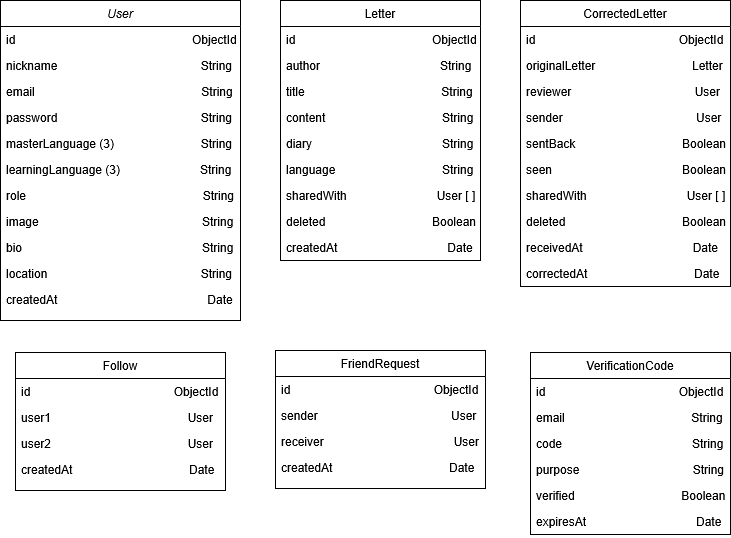
\includegraphics[width=\textwidth]{./imagenes/letterexDB.png}
    \caption{Estructura de Datos}
    \label{fig:letterexDB}
\end{figure}

Un aspecto importante a mencionar en el diseño de estos esquemas es el uso del ObjectId. En MongoDB, cada documento generado recibe de forma automática un campo \texttt{\_id} único de 12 bytes. A diferencia de los ID incrementales de las bases de datos relacionales (SQL), el ObjectId es un identificador hexadecimal que garantiza la unicidad incluso en sistemas distribuidos. En definitiva, el ObjectId es el tipo de dato para los identificadores y cumple dos funciones críticas: la vinculación mediante referencias, permitiendo incluir campos en colecciones que apunten a documentos de otra (por ejemplo, el campo \texttt{originalLetter} en \texttt{CorrectedLetter} es una referencia a un objeto de la colección \texttt{Letter}); y la indexación eficiente, que permite realizar búsquedas rápidas gracias a su generación basada en marcas de tiempo (timestamps).

Cabe destacar que, aunque MongoDB utiliza de forma nativa el campo \texttt{\_id}, en el diagrama y en el consumo de la API se utiliza el término \texttt{id}. Esta transformación se realiza en la capa del Back-end antes de enviar los datos al Front-end, con el fin de ofrecer una interfaz más limpia, estandarizada y desacoplada de las particularidades del motor de base de datos.

A continuación, se describen las colecciones que conforman el sistema.


\subsection{Colección User (Usuarios)}
Representa a los actores principales del sistema, gestionando su identidad y perfil lingüístico.

\begin{itemize}
    \item \textbf{id}: Identificador único del documento.
    \item \textbf{nickname}: \textit{String} que representa el nombre de usuario. Debe ser único en el sistema.
    \item \textbf{email}: \textit{String} con el correo electrónico del usuario, también validado como único, para la gestión de cuentas y posible recuperación de contraseña.
    \item \textbf{password}: \textit{String} que almacena el hash de la contraseña. Por seguridad, no se almacena el texto plano; se utiliza la librería \textbf{bcrypt} con un factor de coste (\textit{salting}) de 10 para cifrar la clave antes de su persistencia. El salting es un parámetro que determina la complejidad computacional del hash para dificultar ataques de fuerza bruta al aumentar el tiempo de procesamiento necesario. Se ha escogido 10 por ser el estándar actual en la industria, aquel que se considera el punto de equilibrio óptimo entre seguridad y rendimiento.
    \item \textbf{masterLanguage (1, 2, 3)}: \textit{Strings} que definen los idiomas que el usuario domina de forma nativa o sólida. Esta decisión de diseño limita a tres el máximo de idiomas maestros por simplicidad técnica y optimización de las búsquedas de revisores.
    \item \textbf{learningLanguage (1, 2, 3)}: Campos equivalentes a los anteriores destinados a los idiomas que el usuario está aprendiendo y sobre los que desea recibir correcciones.
    \item \textbf{role}: Define el nivel de privilegios del usuario (\texttt{Admin} o \texttt{Standard}).
    \item \textbf{image}: \textit{String} que contiene la ruta o nombre del archivo de la imagen de perfil.
    \item \textbf{bio / location}: Campos de texto para la personalización del perfil y ubicación geográfica.
    \item \textbf{createdAt}: Dato de tipo \textit{Date} que registra automáticamente el momento del registro del usuario.
\end{itemize}

\subsection{Colección Letter (Cartas)}
Almacena los textos originales redactados por los usuarios para ser compartidos y corregidos.

\begin{itemize}
    \item \textbf{id}: Identificador único del documento.
    \item \textbf{author}: Referencia al usuario creador del contenido.
    \item \textbf{title / content}: Título y cuerpo del texto de la carta.
    \item \textbf{diary}: String con el diario de la carta. Es una forma de que el usuario pueda organizar sus cartas en diferentes grupos si lo desea.
    \item \textbf{language}: Idioma en el que está redactado el texto.
    \item \textbf{sharedWith}: Array de referencias a la colección \textit{User}, que identifica a los usuarios con permisos de visualización y corrección.
    \item \textbf{deleted}: Booleano utilizado para el borrado lógico, permitiendo ocultar el recurso sin eliminarlo físicamente de la base de datos.
    \item \textbf{createdAt}: Fecha de creación del documento.
\end{itemize}

\subsection{Colección CorrectedLetter (Cartas Corregidas)}
Gestiona la lógica de intercambio y el flujo de revisión entre el autor y el corrector.

\begin{itemize}
    \item \textbf{id}: Identificador único del documento.
    \item \textbf{originalLetter}: Referencia de tipo ObjectId que vincula la corrección con su carta de origen.
    \item \textbf{reviewer / sender}: Referencias a los usuarios que actúan como corrector y receptor, respectivamente.
    \item \textbf{sentBack / seen}: Atributos booleanos que controlan el flujo de estado de la corrección (enviada y leída).
    \item \textbf{receivedAt / correctedAt}: Marcas de tiempo para la trazabilidad del proceso de revisión.
\end{itemize}

\subsection{Colección Follow}
Esta colección gestiona el grafo social de la aplicación, permitiendo establecer vínculos de seguimiento entre los usuarios de la plataforma para facilitar el intercambio de correcciones.

\begin{itemize}
    \item \textbf{id}: Identificador único del documento.
    \item \textbf{user1}: Referencia de tipo \textit{User} que representa al usuario que inicia la relación de seguimiento.
    \item \textbf{user2}: Referencia de tipo \textit{User} que representa al usuario que es seguido.
    \item \textbf{createdAt}: Marca de tiempo de tipo \textit{Date} que registra el momento exacto en el que se estableció la relación entre ambos usuarios.
\end{itemize}

\subsection{Colección FriendRequest}
Esta colección actúa como una capa intermedia para la gestión de relaciones sociales, almacenando las solicitudes de amistad pendientes de resolución por parte del usuario receptor.

\begin{itemize}
    \item \textbf{id}: Identificador único de la solicitud de amistad (\texttt{ObjectId}).
    \item \textbf{sender}: Referencia de tipo \textit{User} que identifica al usuario que emite la petición.
    \item \textbf{receiver}: Referencia de tipo \textit{User} que identifica al destinatario de la solicitud.
    \item \textbf{createdAt}: Marca de tiempo de tipo \textit{Date} que registra el momento en el que se envió la petición.
\end{itemize}

Es importante destacar la naturaleza efímera de esta colección dentro de la lógica del sistema: una vez que el usuario \texttt{receiver} interactúa con la petición, el documento es eliminado de la base de datos. Si la solicitud es aceptada, se procede a la creación de un nuevo registro en la colección \textbf{Follow} para consolidar el vínculo; en caso de ser rechazada, el documento simplemente desaparece, garantizando así que la base de datos no mantenga información transitoria innecesaria.

\subsection{Colección VerificationCode}
Se trata de una entidad de apoyo diseñada para gestionar la seguridad en procesos críticos, como la validación de correos electrónicos durante el registro o la recuperación de credenciales.

\begin{itemize}
    \item \textbf{id}: Identificador único del documento de verificación (\texttt{ObjectId}).
    \item \textbf{email}: \textit{String} que contiene la dirección de correo electrónico a la que se vincula el código de seguridad.
    \item \textbf{code}: \textit{String} que almacena el código de 6 números temporal generado por el sistema. Al igual que las contraseñas, estos códigos se almacenan en forma de hash con el mismo salting.
    \item \textbf{purpose}: \textit{String} que describe la finalidad del código, pudiendo ser ``password\_reset'' o ``register''.
    \item \textbf{verified}: Valor booleano que indica si el código ya ha sido utilizado y validado con éxito por el usuario.
    \item \textbf{expiresAt}: Campo de tipo \textit{Date} que define el momento de caducidad del código. Este campo actúa como un índice \textbf{TTL} (\textit{Time To Live}) que se configura con Mongoose para permitir que MongoDB elimine el documento de forma automática una vez alcanzada esta fecha para garantizar la seguridad. El TTL en este caso, dado que estos códigos se utilizan de forma inmediata (al registrar una nueva cuenta o solicitar una nueva contraseña), es de 7 minutos.
\end{itemize}
